\section{Architettura dell'ATmega32}
L'ATmega32 ha una architettura di tipo Harvard. In particolare abbiamo:
\begin{figure}[H]
    \centering
    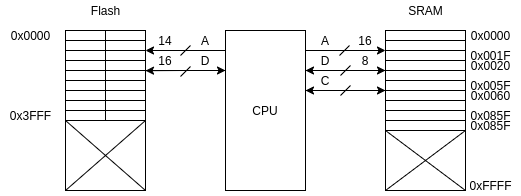
\includegraphics[width=330px]{images/3_Architettura_ATmega32/ATmega32.png}
\end{figure}

\subsection{Struttura della flash}
La memoria flash è composta da 16k righe di 16 bit, oppure 32k righe da 8 bit.
Questo 32k da il nome al microcontrollore.
Dato che gli accessi sono fatti a 16 bit sarebbe più corretto dire che la memoria è composta da 16 Kword piuttosto che da 32 Kbyte.
La memoria flash è occupata dal programma!

E' implementata dall'indirizzo 0x0000 fino all'indirizzo 0x3FFF, il resto dello spazio di indirizzamento è lasciato per utilizzi futuri. Si noti infatti che i bit di indirizzo sono 14 e non 16.

\subsection{Struttura della SRAM}
La SRAM può essere letta e scritta a piacere, è di fatto una RAM, quindi memoria volatile.
La memoria SRAM è più costosa in termini di transistori (6 transistori rispetto a 1 della flash), più grande sul chip ma è veloce. E' organizzata in celle da 8 bit ed è così segmentata:
\begin{itemize}
    \item 0x0000 - 0x001F: copia dei registri
    \item 0x0020 - 0x005F: periferiche
    \item 0x0060 - 0x085F: RAM
    \item 0x0860 - 0xFFFF: non implementata
\end{itemize}

Tra le periferiche si hanno i pin GPIO, cioè una periferica che si connette da una parte allo spazio di memoria e dall'altra ha dei pin che possono essere impostati a livello logico alto o a livello logico basso, sono utilizzati per interagire con il mondo esterno. Altre periferiche sono periferiche di comunicazione (SPI, I$^{2}$C, ecc).

Questo modello è detto \emph{I/O mappato in memoria} in quanto appunto le periferiche sono accessibili come fossero vera e propria memoria.

NB: se scrivo nella memoria non connessa è come se non avessi fatto niente, se leggo da quegli indirizzi leggo 0xFF, si dice che \emph{fallisce in silenzio}.


\subsection{CPU}
Le componenti fondamentali della CPU sono:
\begin{itemize}
    \item Decodificatore delle istruzioni: una volta letta l'istruzione dalla flash si occupa di decifrarla e configurare lo stato interno del processore per eseguirla.
    \item ALU: è l'unità aritmetico-logica, si occupa di eseguire le operazioni matematiche (somma, differeza, shift, ecc) e quelle logiche (comparazione, or, and). Non ha la moltiplicazione.
    \item Moltiplicatore: è un aggiunta alla ALU per poter eseguire le moltiplicazioni. E' stato aggiunto nella versione Mega dell'architettura.
    \item Registri r0-r31: sono memorie interne al processore da 1 byte, sono memorie volatili. Le operazioni di manipolazione dei dati vanno fatte esclusivamente all'interno dei registri, quindi servono e ne servono molti. Questi registri sono anche copiati in memoria, modificando un registro modifico la memoria, modificando la memoria modifico i registri:
    \begin{verbatim}
        MOV r7, r9          # copia r9 in r7
        STS 0x0007, r9      # scrivi r9 all'indirizzo 0x0007
    \end{verbatim}
    fanno la stessa cosa!
    La lettura dai registri non è distruttiva, la scrittura invece sovrascrive il valore precedente con quello nuovo!
\end{itemize}


